\section{SOFTWARE}

\subsection{Description of the implementation}
The solution is implemented with a \acrfullr{fsm} with three states, starting from a TEST mode and switching to the next with the USER button of the L072CZ. A common factor of these states is that in all of them, all the data from the sensors need to be obtained.

To solve the need for asynchronous data obtention from the sensors, the solution is based on threads and queues. There are three threads:
\begin{itemize}
    \item Main thread with the \acrshort{fsm}.
    \item I2C thread.
    \item GPS thread.
\end{itemize}

These thread are signalized to wake up when new measurements are needed by the \acrshort{fsm}. When all the information is collected, the information goes to the main thread through a Mbed-OS queue. When all the necessary 
information is obtained, the main thread sends the new data to the computer and waits a set amount of time to start the process again.
\subsection{Module, threads and communications design}
To make the design modular, each hardware element is implemented in a single module, with a \texttt{.cpp} and a \texttt{.h} file.

Considering the asynchronous nature of some of the sensors, the i2c sensors were implemented in an independent thread and the GPS in another thread. In the , the final module design as well as the threads implemented 
can be seen in \autoref{fig:moduleDiagram}.
\begin{figure}[H]
    \centering
    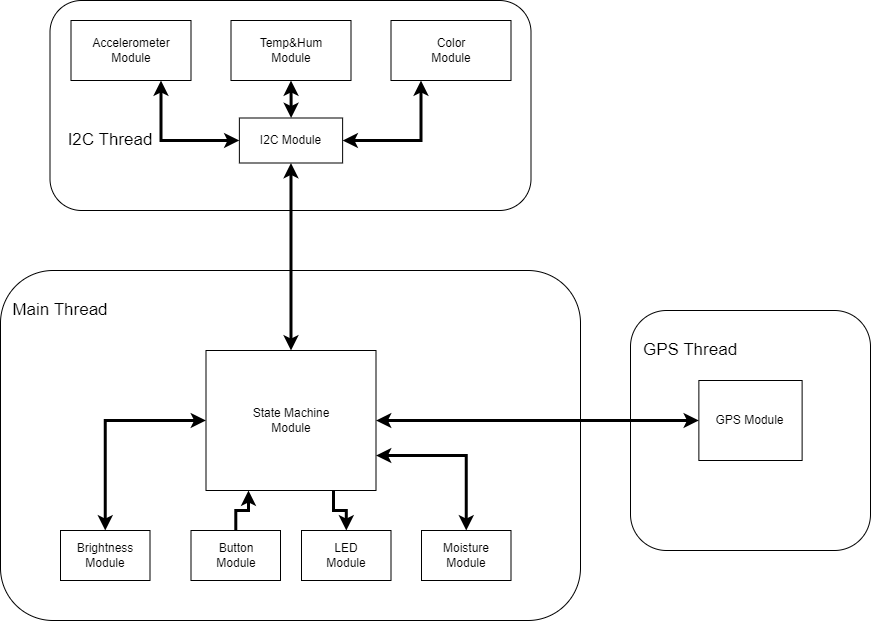
\includegraphics[width=0.9\textwidth]{images/4/softdiagram.png}
    \caption{Module diagram of the software and threads}
    \label{fig:moduleDiagram}
\end{figure}

For the communications from the control to the \acrshort{i2c} and the GPS, there was only need to indicate to the \acrshort{i2c} and GPS threads to launch all the necessary measurements on demand, so in this case signals were used.
For the data flowing from the sensors to the control module, as signals in a processor are limited(in our case 32 bit register for signals), a queue was used.

A queue is a thread safe mechanism of low level that implements a FIFO buffer with a in endpoint and an out endpoint. Any process can insert new data into the queue with a blocking call and the same can be done to extract the data. Finally, the data 
inside the queue is managed by the queue itself(at least in the implementation in Mbed-OS).

To reduce the memory usage, only one queue was defined for the whole system. With this done, extra logic was needed to differentiate messages from different sensors, so a message structure was defined like a pseudo-protocol. This can be seen in the \hyperref[appendix]{appendix}.

\subsection{State machine module}
The state machine module controls the whole system, 
\subsection{I2C module}

\subsection{GPS module}
\clearpage
\subsection{Code size}
For the code size of the project, the information resulting from the compilation in Mbed Studio is presented in the next figures. It must be noted that no changes to the default compilation profiles were done.
\begin{figure}[H]
    \centering
    \begin{subfigure}[t]{0.45\textwidth}
        \centering
        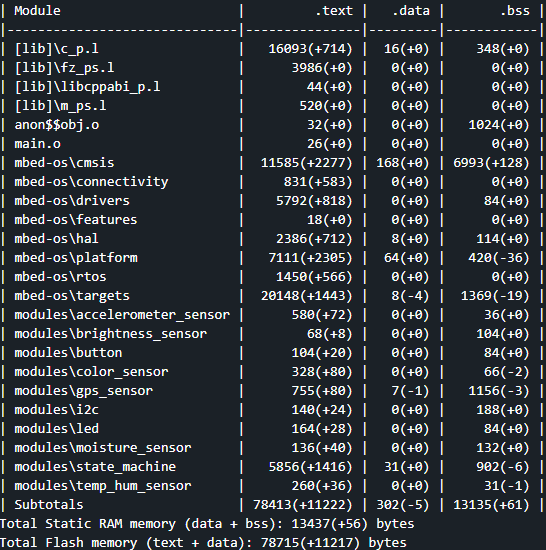
\includegraphics[width=0.95\textwidth]{images/4/Debug.png}
        \caption{Debug compilation}
    \end{subfigure}
    \begin{subfigure}[t]{0.45\textwidth}
        \centering
        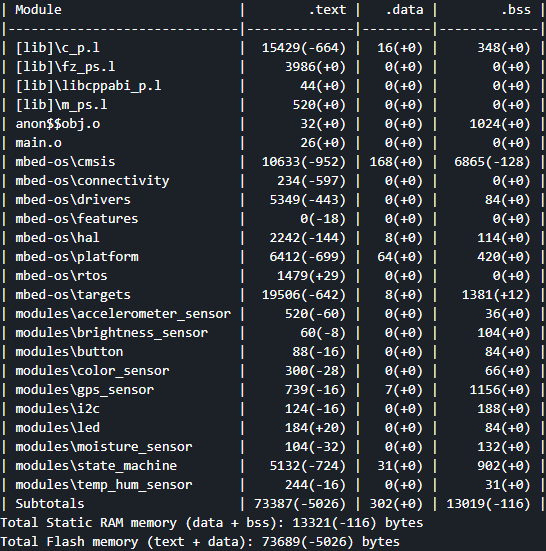
\includegraphics[width=0.95\textwidth]{images/4/Develop.png}
        \caption{Develop compilation}
    \end{subfigure}
    \begin{subfigure}[t]{0.45\textwidth}
        \centering
        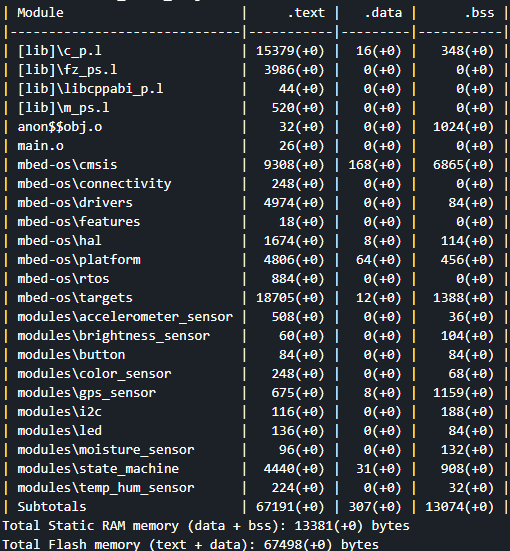
\includegraphics[width=0.95\textwidth]{images/4/Release.png}
        \caption{Release compilation}
    \end{subfigure}
    \caption{Code size and module size for every compilation profile}
    \label{fig:compilation}
\end{figure}

The most heavy modules in terms of size were:
\begin{enumerate}
    \item The state machine with 476 lines of code.
    \item The GPS with 86 lines of code, but with a parsing of a string, which needs lot of resources.
\end{enumerate}
